\graphicspath{{figures/Design/IPController/}}
\chapter{Design of the Inverted Pendulum Controller}\label{sec:IPController}
The goal of the controller is to balance the rocket body in an upright position. 

As seen in the modeling of the rocket, the system presents poles and zeros in the origin of the pole-zero plot. The system is unstable and goes to infinity on the imaginary axis. To solve this problem a zero could be added at a higher frenquency to attract the poles.

				% Figure of original tf
%\begin{figure}[htbp]
%	\centering
%	
%		\includegraphics[width=\textwidth]{figures/appendix/Rocket/initial_transfer_function}
%		\caption{Root locus of the initial rocket angle transfer function.}
%		\label{fig:locus1tf}
%	
%\end{figure}

However the real system is influenced by the servomotors. The transfer function of the servomotors adds a pole, resulting in an unstable system moving towards infinity on the imaginary axis. 
				
				% Figure of tf + servo
%\begin{figure}[htbp]
%	\centering
%	\begin{subfigure}{0.45\textwidth}
%		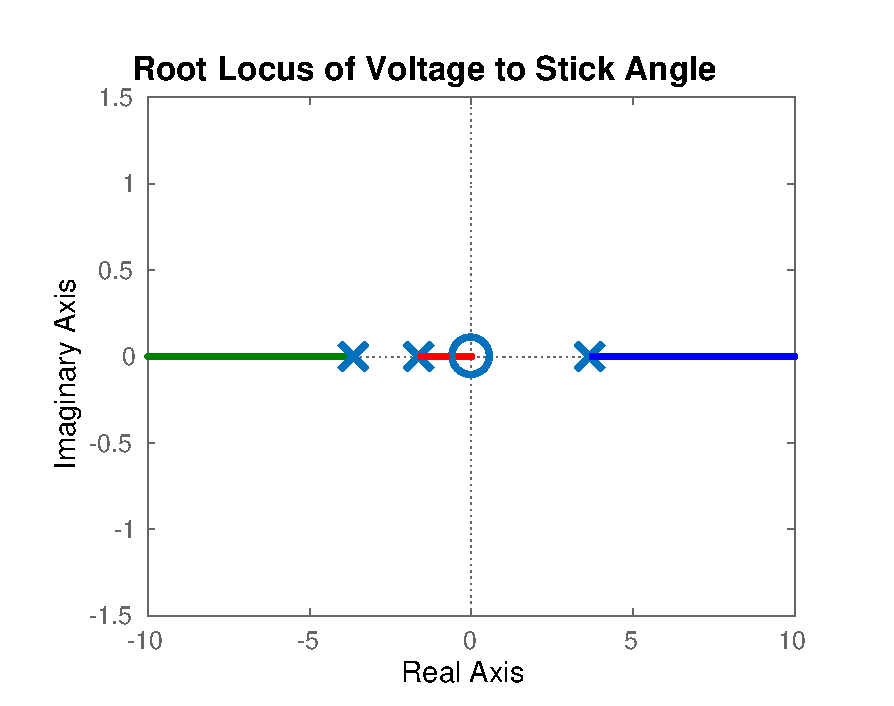
\includegraphics[width=\textwidth]{rlocusplus}
%		\caption{Positive gain.}
%		\label{fig:locusIP}
%	\end{subfigure}
%	\begin{subfigure}{0.45\textwidth}
%		\centering
%		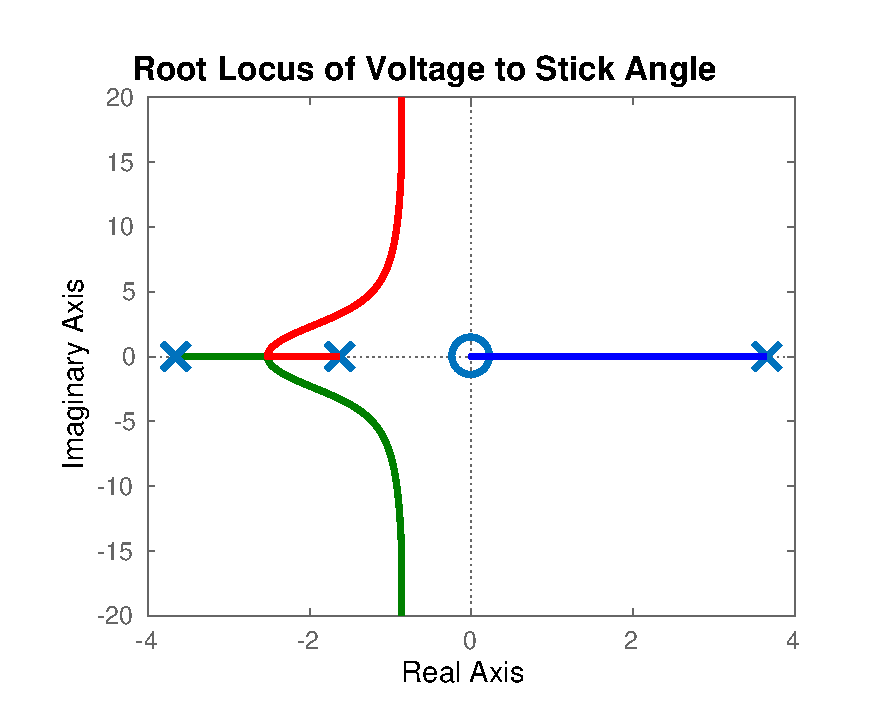
\includegraphics[width=\textwidth]{rlocusminus}
%		\caption{Negative gain.}
%		\label{fig:locusNegative}
%	\end{subfigure}
%	\caption{Root locus of the inverted pendulums transfer function.}
%\end{figure}

To direct the root locus to a stable state, a controller C1, adding a zero and a pole on the left side, is implemented. The zero of the controller is chosen to be near the system in order to attract the poles. The pole of the controller is set at high frequency to not temper with the system. 

				% Figure of tf + servo + C1, and zoom of tf + servo + C1
%\begin{figure}[htbp]
%	\centering
%	\begin{subfigure}{0.45\textwidth}
%		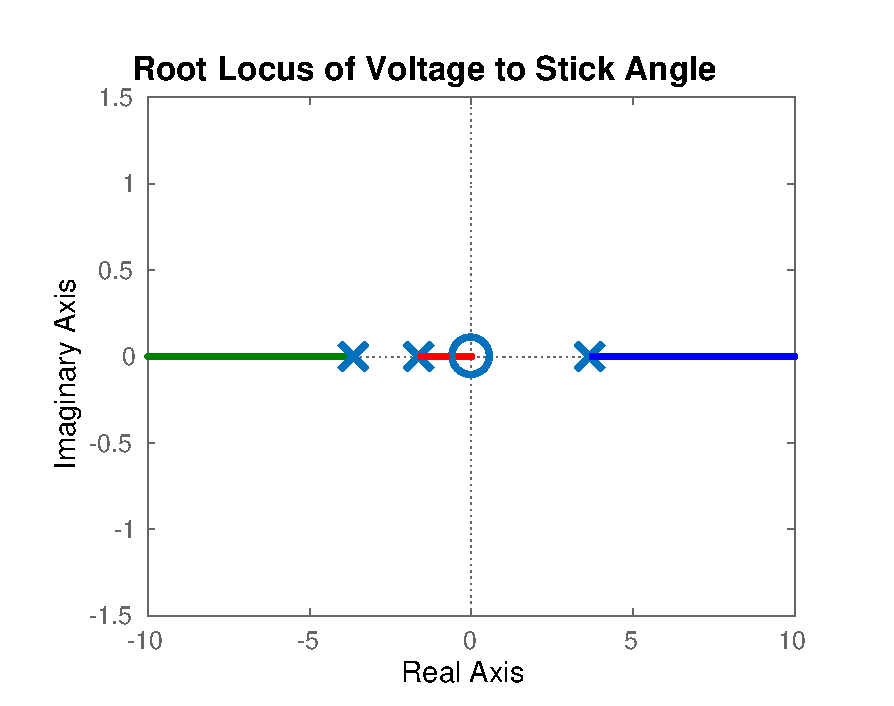
\includegraphics[width=\textwidth]{rlocusplus}
%		\caption{Positive gain.}
%		\label{fig:locusIP}
%	\end{subfigure}
%	\begin{subfigure}{0.45\textwidth}
%		\centering
%		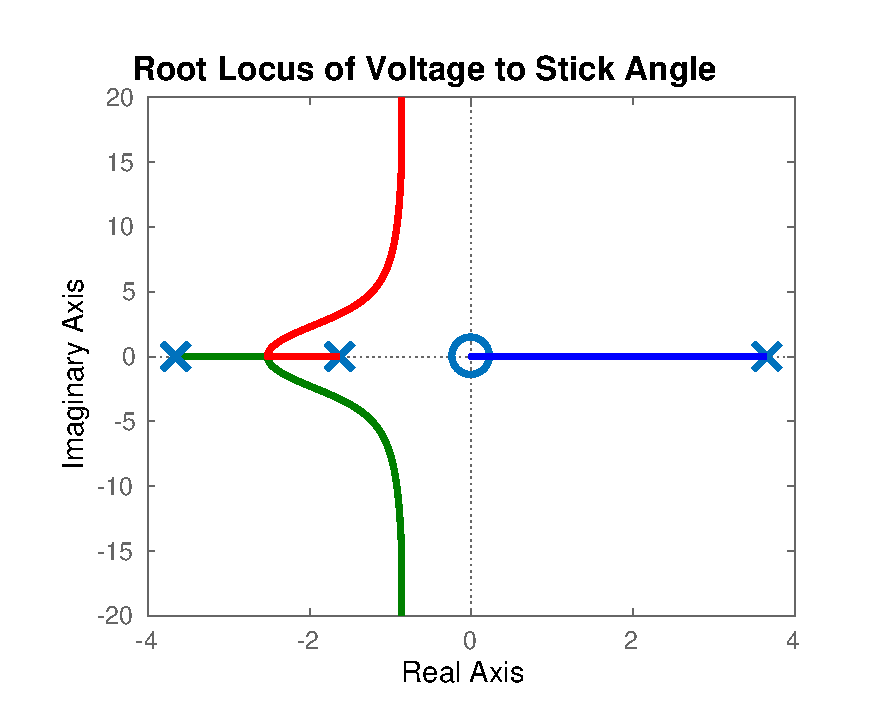
\includegraphics[width=\textwidth]{rlocusminus}
%		\caption{Negative gain.}
%		\label{fig:locusNegative}
%	\end{subfigure}
%	\caption{Root locus of the inverted pendulums transfer function.}
%\end{figure}

Another controller C2 is needed to attract the two poles going to infinity along the imaginary axis. The pole and zeros of C2 are set at higher frequencies than the first controller C1. 

				% Figure of final tf with controllers 
%\begin{figure}[htbp]
%	\centering
%	\begin{subfigure}{0.45\textwidth}
%		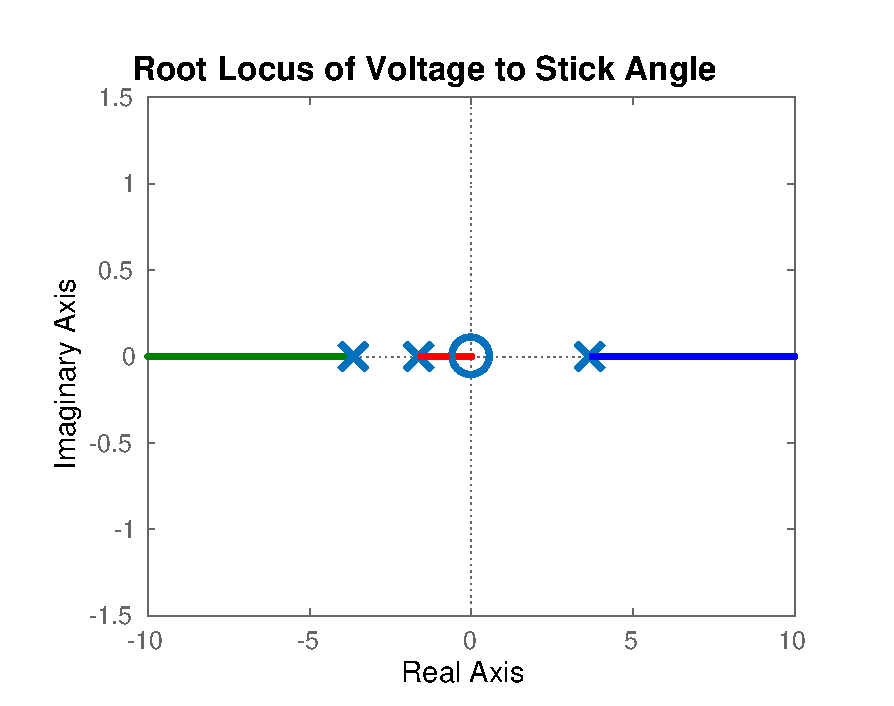
\includegraphics[width=\textwidth]{rlocusplus}
%		\caption{Positive gain.}
%		\label{fig:locusIP}
%	\end{subfigure}
%	\begin{subfigure}{0.45\textwidth}
%		\centering
%		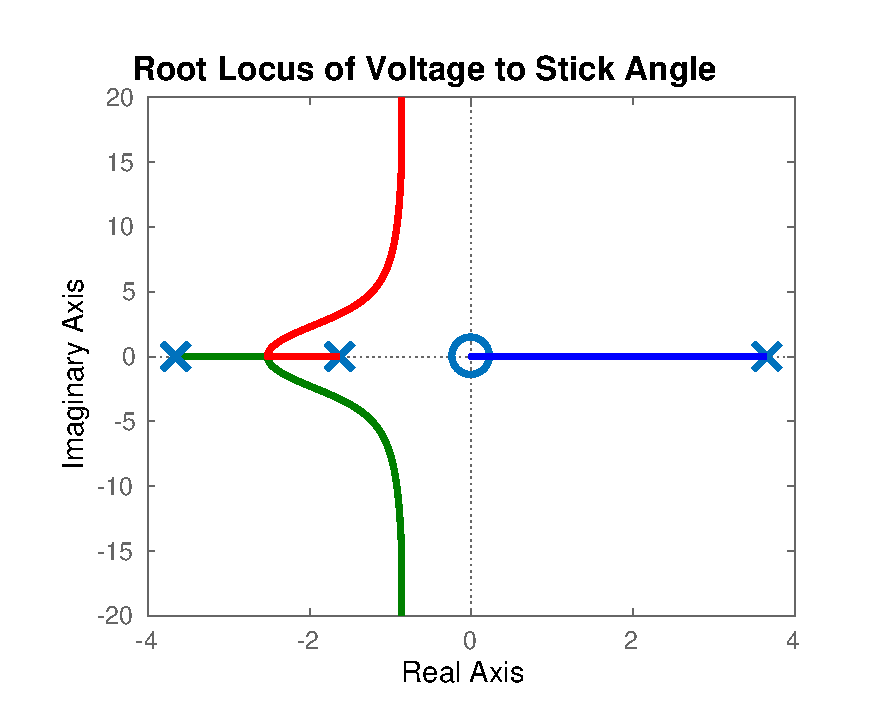
\includegraphics[width=\textwidth]{rlocusminus}
%		\caption{Negative gain.}
%		\label{fig:locusNegative}
%	\end{subfigure}
%	\caption{Root locus of the inverted pendulums transfer function.}
%\end{figure}

The rocket requires a fast settling time and rise time in order to act as soon as possible and control the rocket's stability. Lead compensaters enable the modulation of the rise time, but impact the overshoot. The overshoot is considered as an inferrior error, being in part countered by the play of the gimbal system. 

To improve the setling time, the gain is set at %2.15 * 10^3.
This value is chosen by observing the root locus and the gain of a set point.

				% Figure of chosen point, and of final tf with 2.15*10^3
%\begin{figure}[htbp]
%	\centering
%	\begin{subfigure}{0.45\textwidth}
%		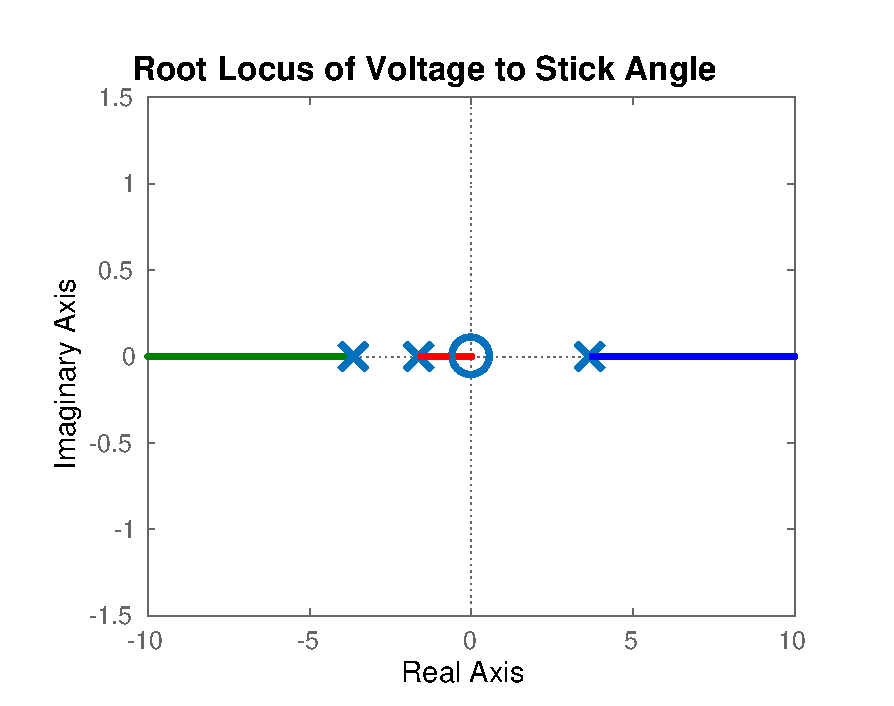
\includegraphics[width=\textwidth]{rlocusplus}
%		\caption{Positive gain.}
%		\label{fig:locusIP}
%	\end{subfigure}
%	\begin{subfigure}{0.45\textwidth}
%		\centering
%		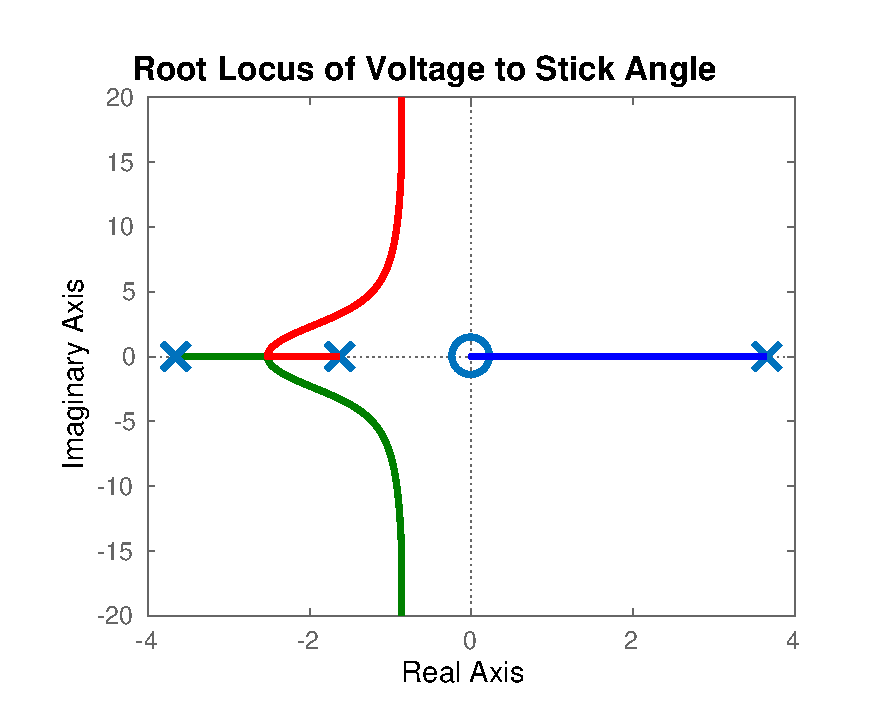
\includegraphics[width=\textwidth]{rlocusminus}
%		\caption{Negative gain.}
%		\label{fig:locusNegative}
%	\end{subfigure}
%	\caption{Root locus of the inverted pendulums transfer function.}
%\end{figure}


The servomotors can have a faster rising time according to the step response of the servomotors. The gain is then doubled to improve the rise time and setling time.

%\begin{table}[htbp]
%	\centering
%	\caption{Simulated rising time.}
%	\label{RPMData}
%	\begin{tabular}{llll}
%		Transfer function & Rise time{(}s{)} \\ \hline  \rowcolor{lightGrey}
%		Gain of 2.15*10^3     & 0.1669	\\  
%		Servomotors     & 0.0589     \\  
%		\rowcolor{lightGrey}           
%		Gain of 5*10^3     & 0.0854          \\     
%	\end{tabular}
%\end{table}

				% Figure of final tf with 5*10^3
%\begin{figure}[htbp]
%	\centering
%	\begin{subfigure}{0.45\textwidth}
%		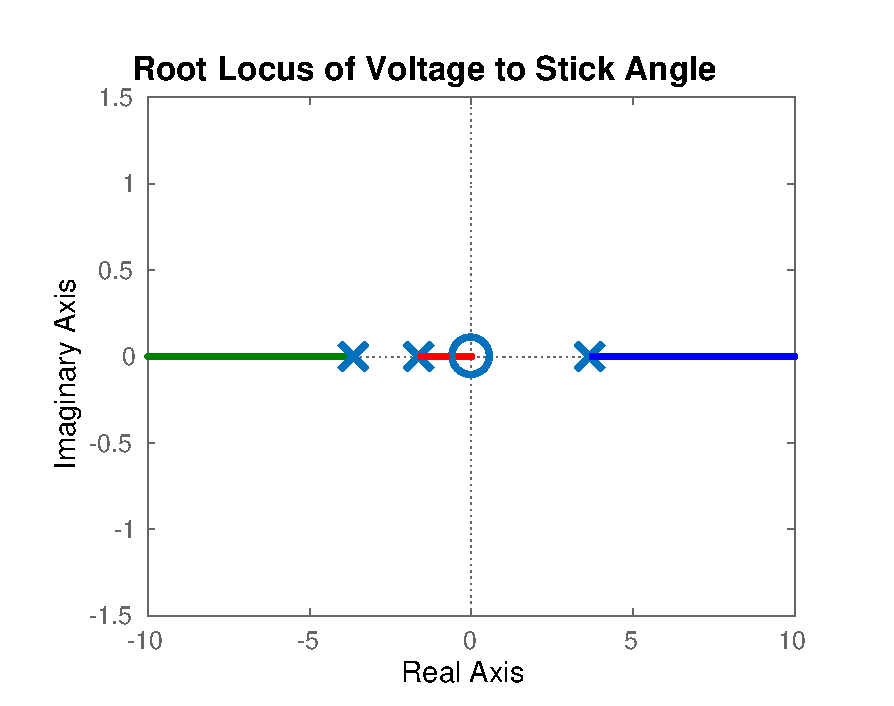
\includegraphics[width=\textwidth]{rlocusplus}
%		\caption{Positive gain.}
%		\label{fig:locusIP}
%	\end{subfigure}
%	\begin{subfigure}{0.45\textwidth}
%		\centering
%		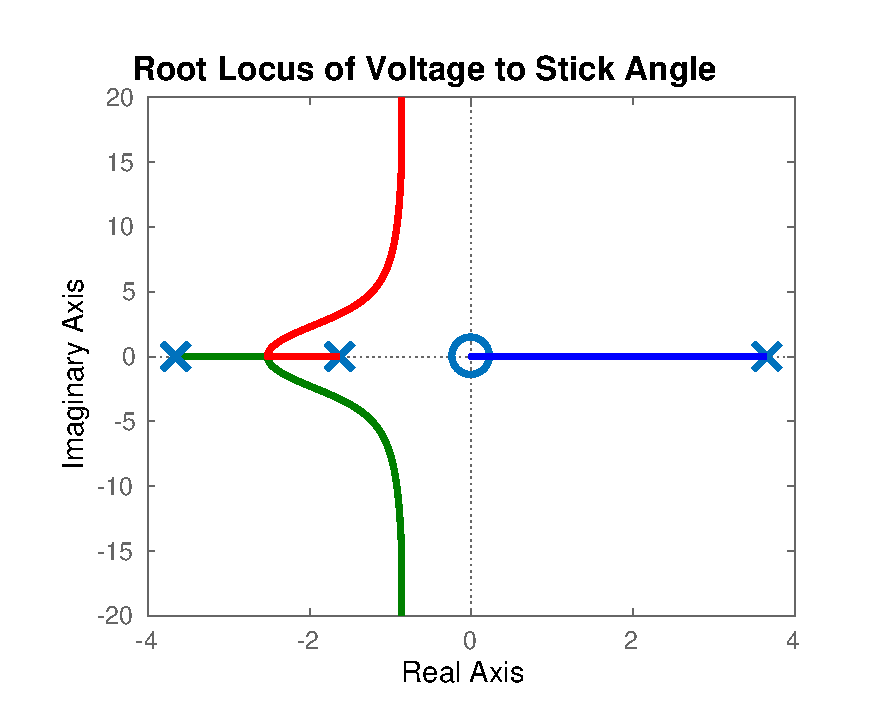
\includegraphics[width=\textwidth]{rlocusminus}
%		\caption{Negative gain.}
%		\label{fig:locusNegative}
%	\end{subfigure}
%	\caption{Root locus of the inverted pendulums transfer function.}
%\end{figure}


The frequency correponds to a complete rotation of the servomotors. At low frequency a delay is observed. However the system functions at low speed. This implies that the delay has a tempered effect on the system. Higher frequencies are not physicaly possible and do not need to be compensated.

				% Figure of final tf bodepoint
%\begin{figure}[htbp]
%	\centering
%	\begin{subfigure}{0.45\textwidth}
%		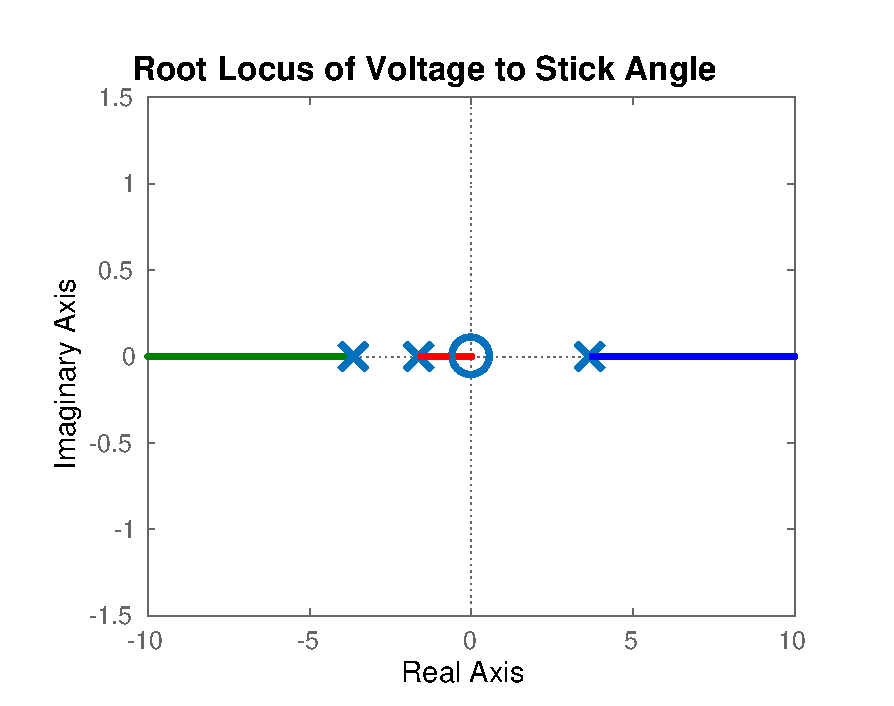
\includegraphics[width=\textwidth]{rlocusplus}
%		\caption{Positive gain.}
%		\label{fig:locusIP}
%	\end{subfigure}
%	\begin{subfigure}{0.45\textwidth}
%		\centering
%		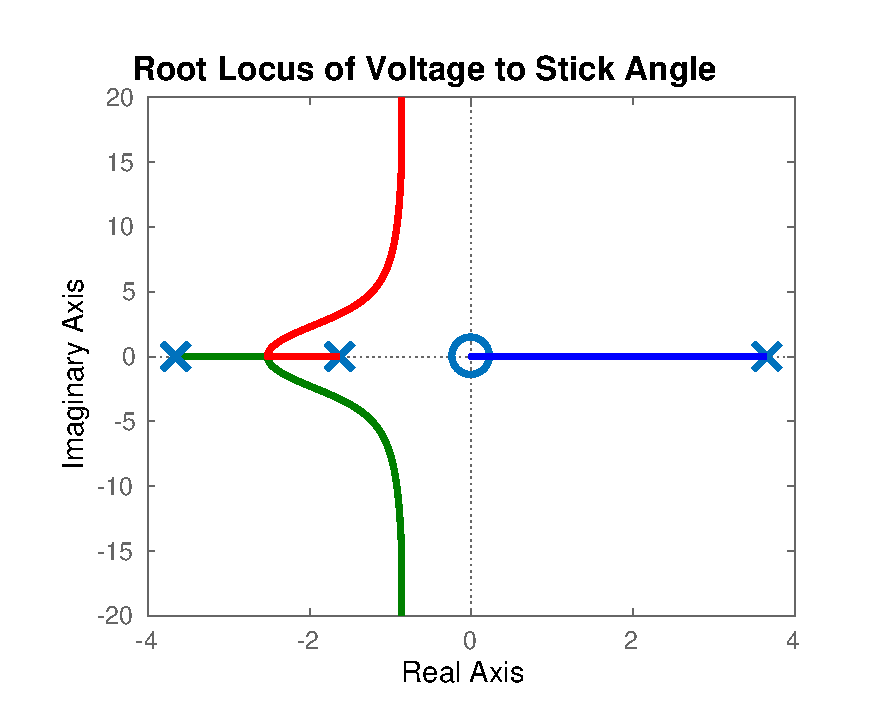
\includegraphics[width=\textwidth]{rlocusminus}
%		\caption{Negative gain.}
%		\label{fig:locusNegative}
%	\end{subfigure}
%	\caption{Root locus of the inverted pendulums transfer function.}
%\end{figure}